\section{Serielle Datenübertragung - SPI}

\subsection{SPI Basics}
\subsubsection{Kommunikationsmodi}
\begin{itemize}
    \item Simplex: Unidirektional, nur eine Richtung
    \item Halb-Duplex: Bidirektional, aber nur eine Richtung zur gleichen Zeit
    \item Vollduplex: Bidirektional, beide Richtungen gleichzeitig
\end{itemize}

\subsubsection{Timing}
\begin{itemize}
    \item Synchron: Beide Geräte verwenden denselben Takt (meistenfalls Master)
    \item Asynchron: Jedes Gerät hat seinen eigenen Takt
\end{itemize}

\subsubsection{Synchrone serielle Kommunikation}
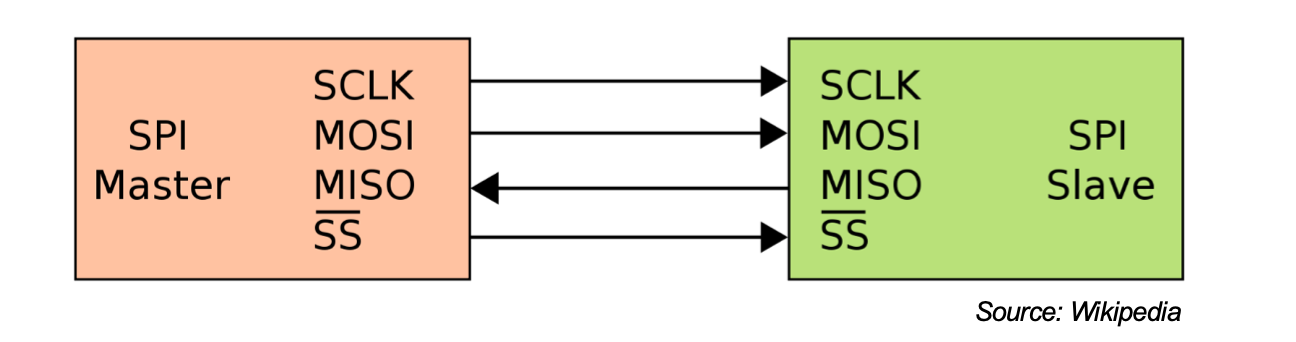
\includegraphics[width=0.3\textwidth]{sections/images/spi_synchron.png}
\begin{itemize}
    \item Full-Duplex
    \item Master generiert Takt (SCLK) und initiiert Datenübertragung via Slave Select ($\overline{SS}=0$)
    \item MOSI: Master Out Slave In
    \item MISO: Master In Slave Out
\end{itemize}

Dies funktioniert auch mit mehreren Slaves, wobei der Master für jeden Slave ein eigenes Slave Select Signal hat. Die Slaves, welche nicht selektiert sind, haben jeweils $\overline{SS}=1$, während der selektierte Slave $\overline{SS}=0$ hat. Der Slave Output ist hochohmig, wenn er nicht selektiert ist.

\subsection{SPI Modi}
\begin{itemize}
    \item TX auf stellt Daten auf der 'Toggling Edge' bereit
    \item RX auf liest Daten auf der 'Sampling Edge'
\end{itemize}

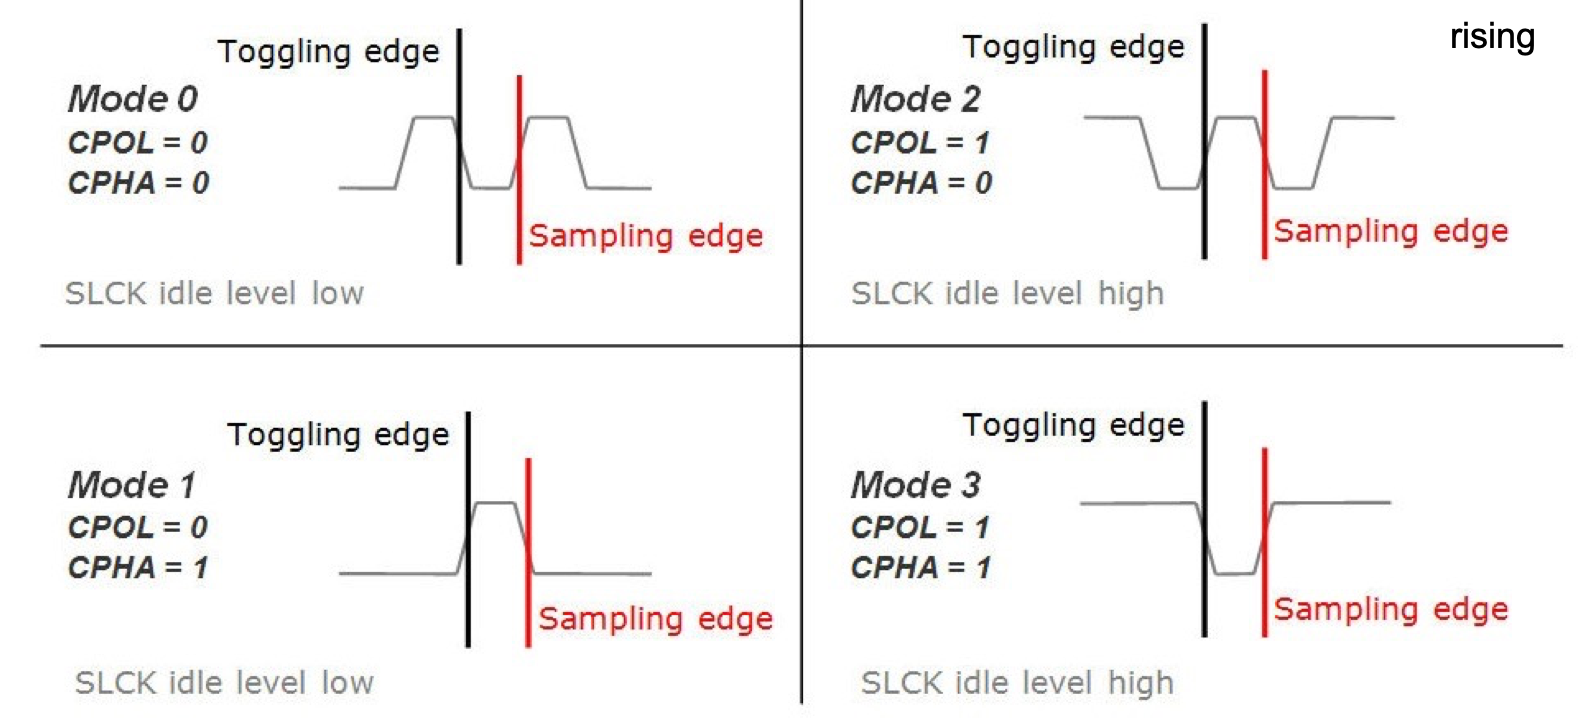
\includegraphics[width=0.3\textwidth]{sections/images/spi_mode1.png}
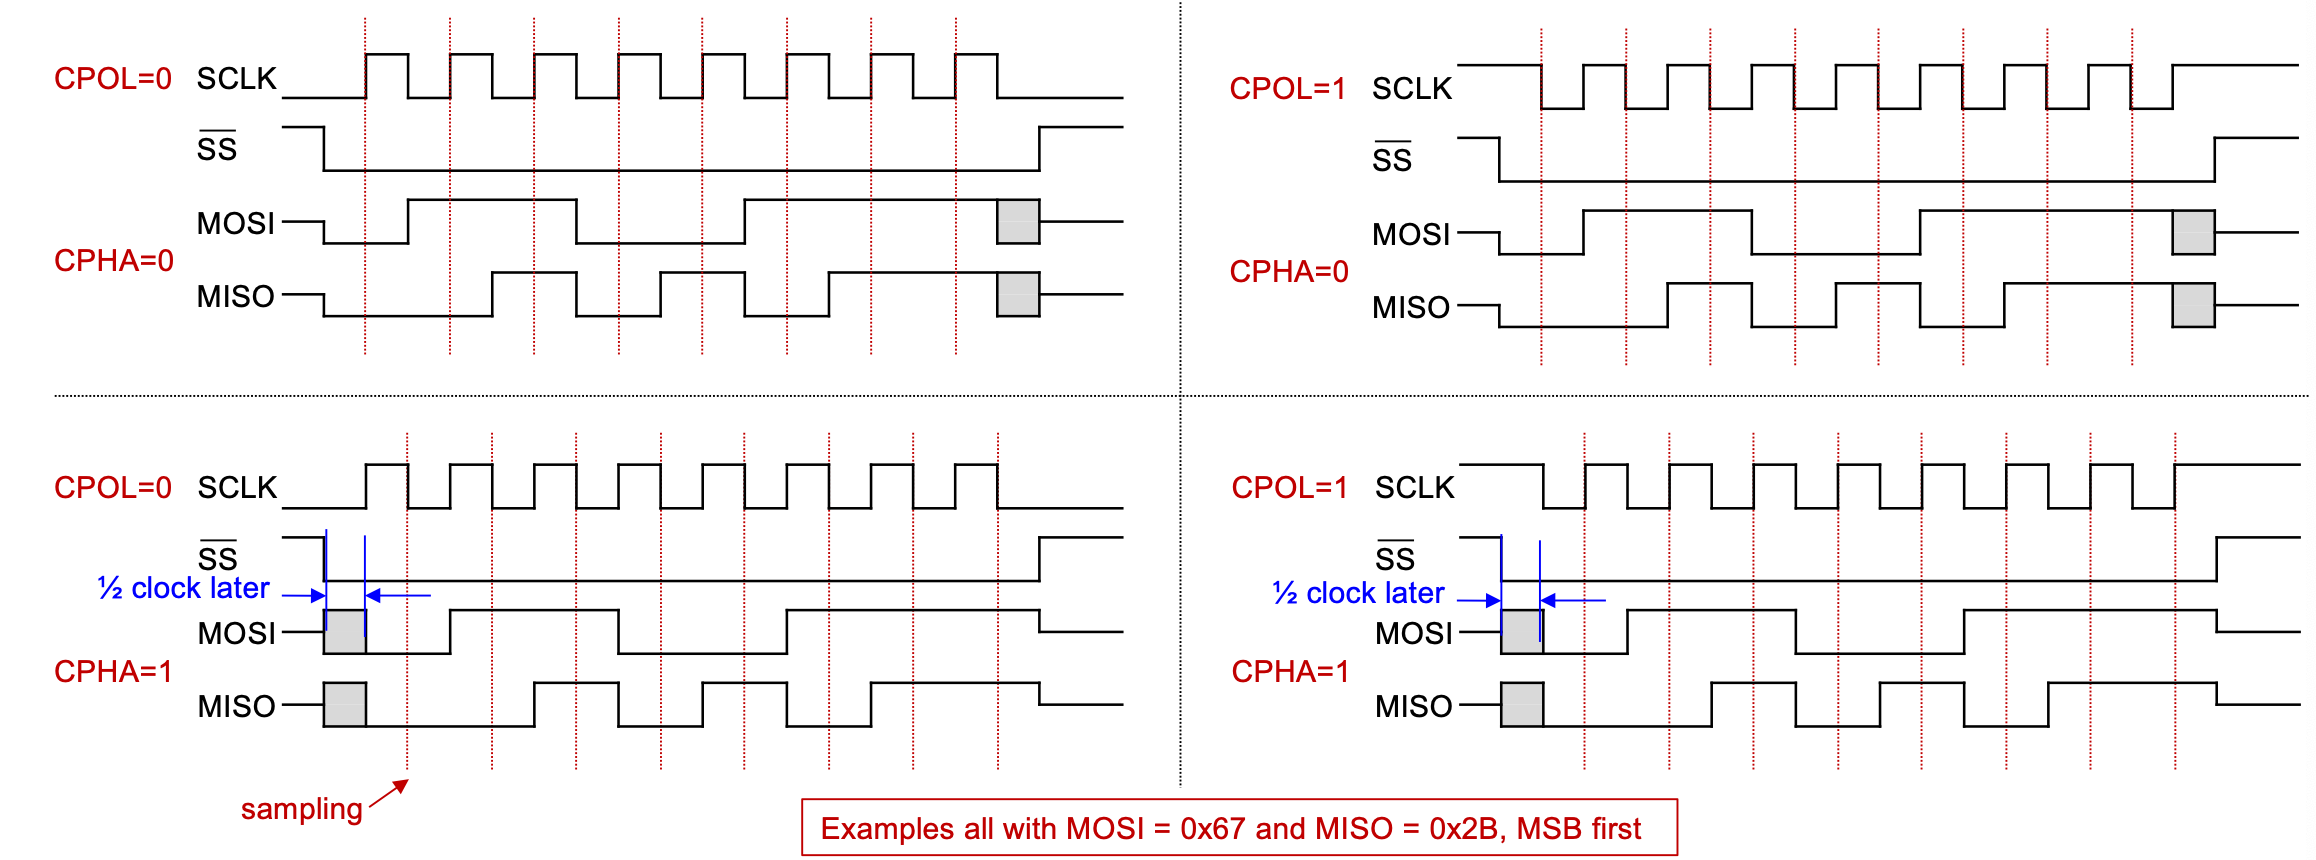
\includegraphics[width=0.3\textwidth]{sections/images/spi_mode2.png}

\subsection{SPI Timing-Diagramm}
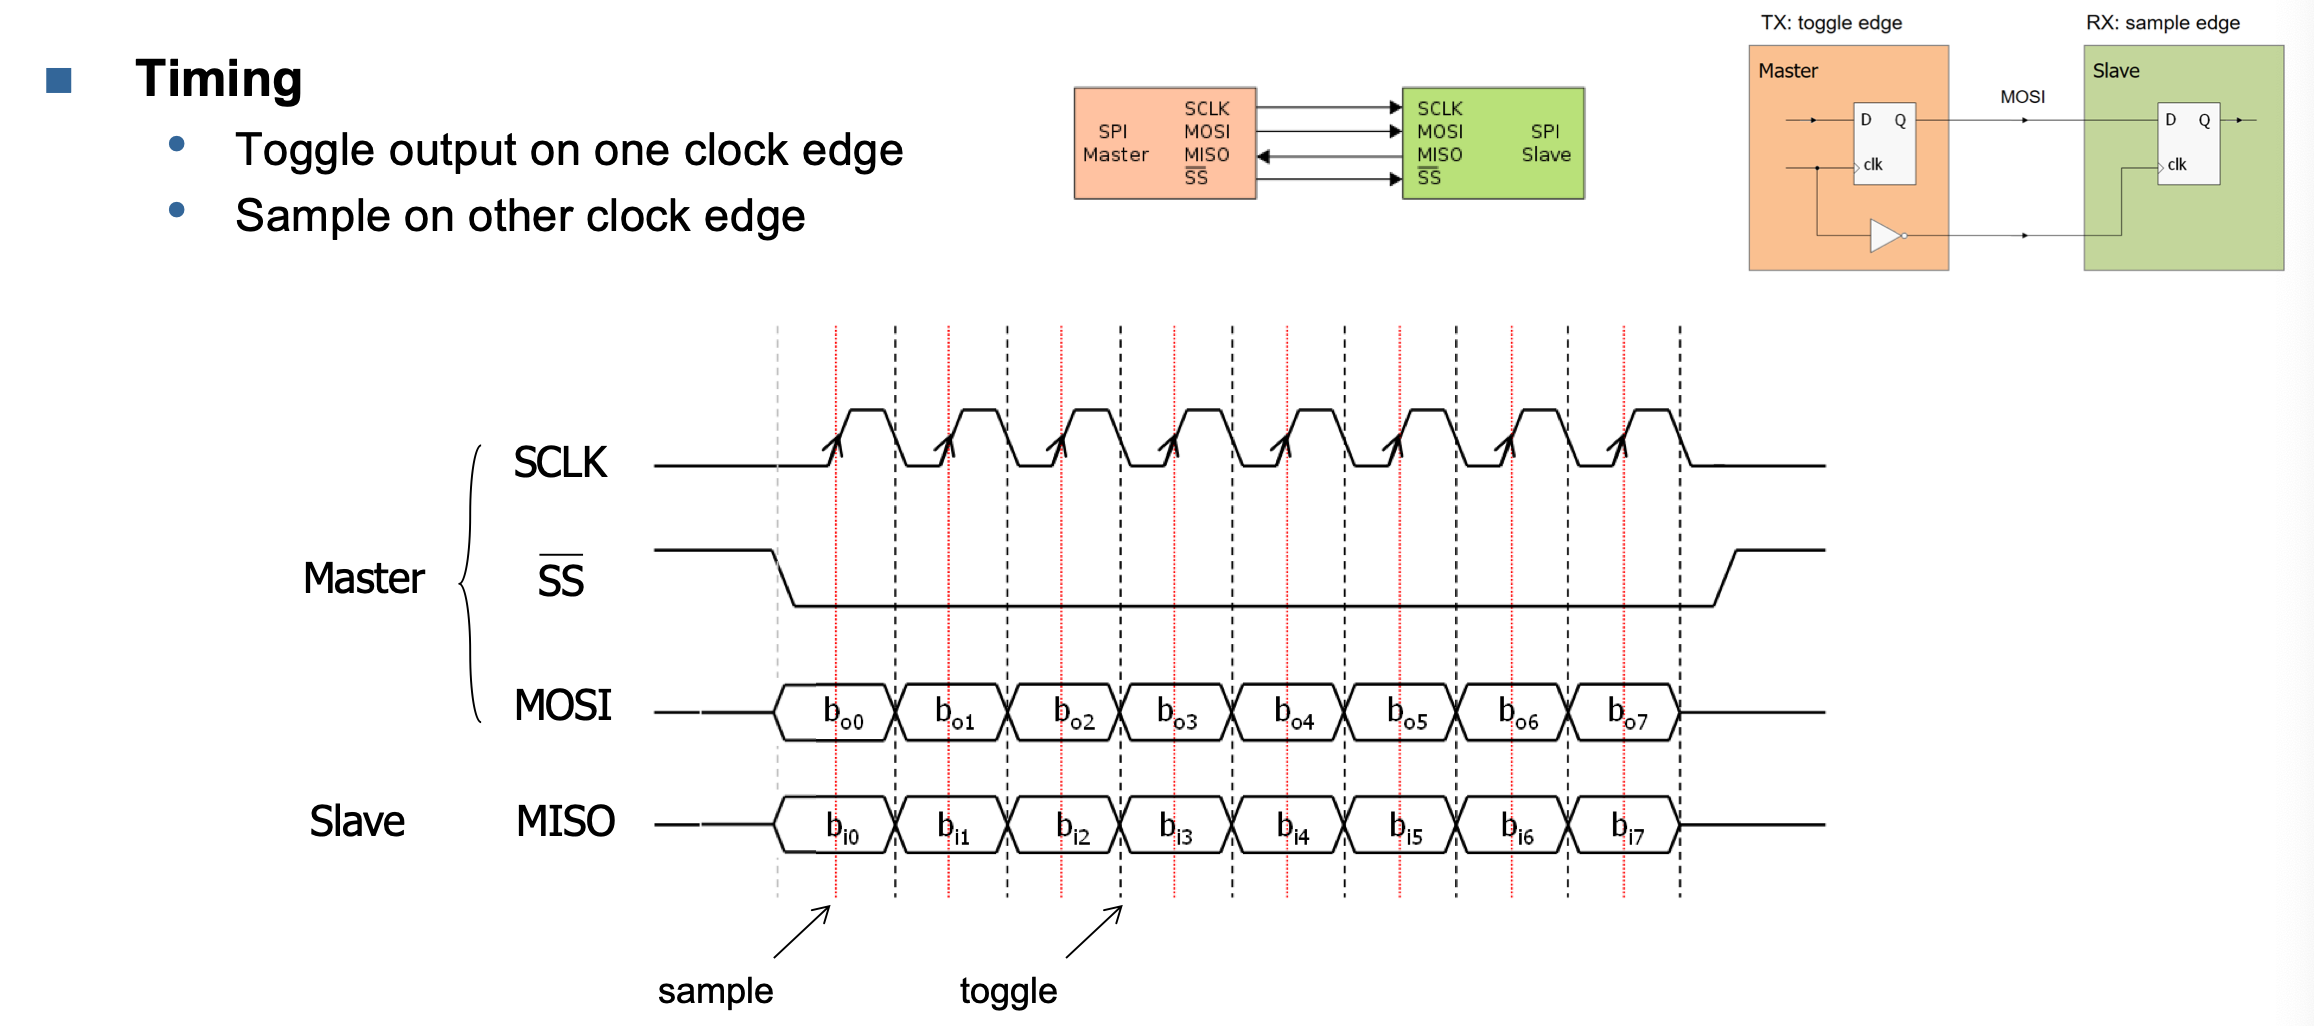
\includegraphics[width=0.3\textwidth]{sections/images/spi_timing.png}

\subsection{Wie wird SPI von der Software auf dem STM32F4-Discovery-Board verwendet?}
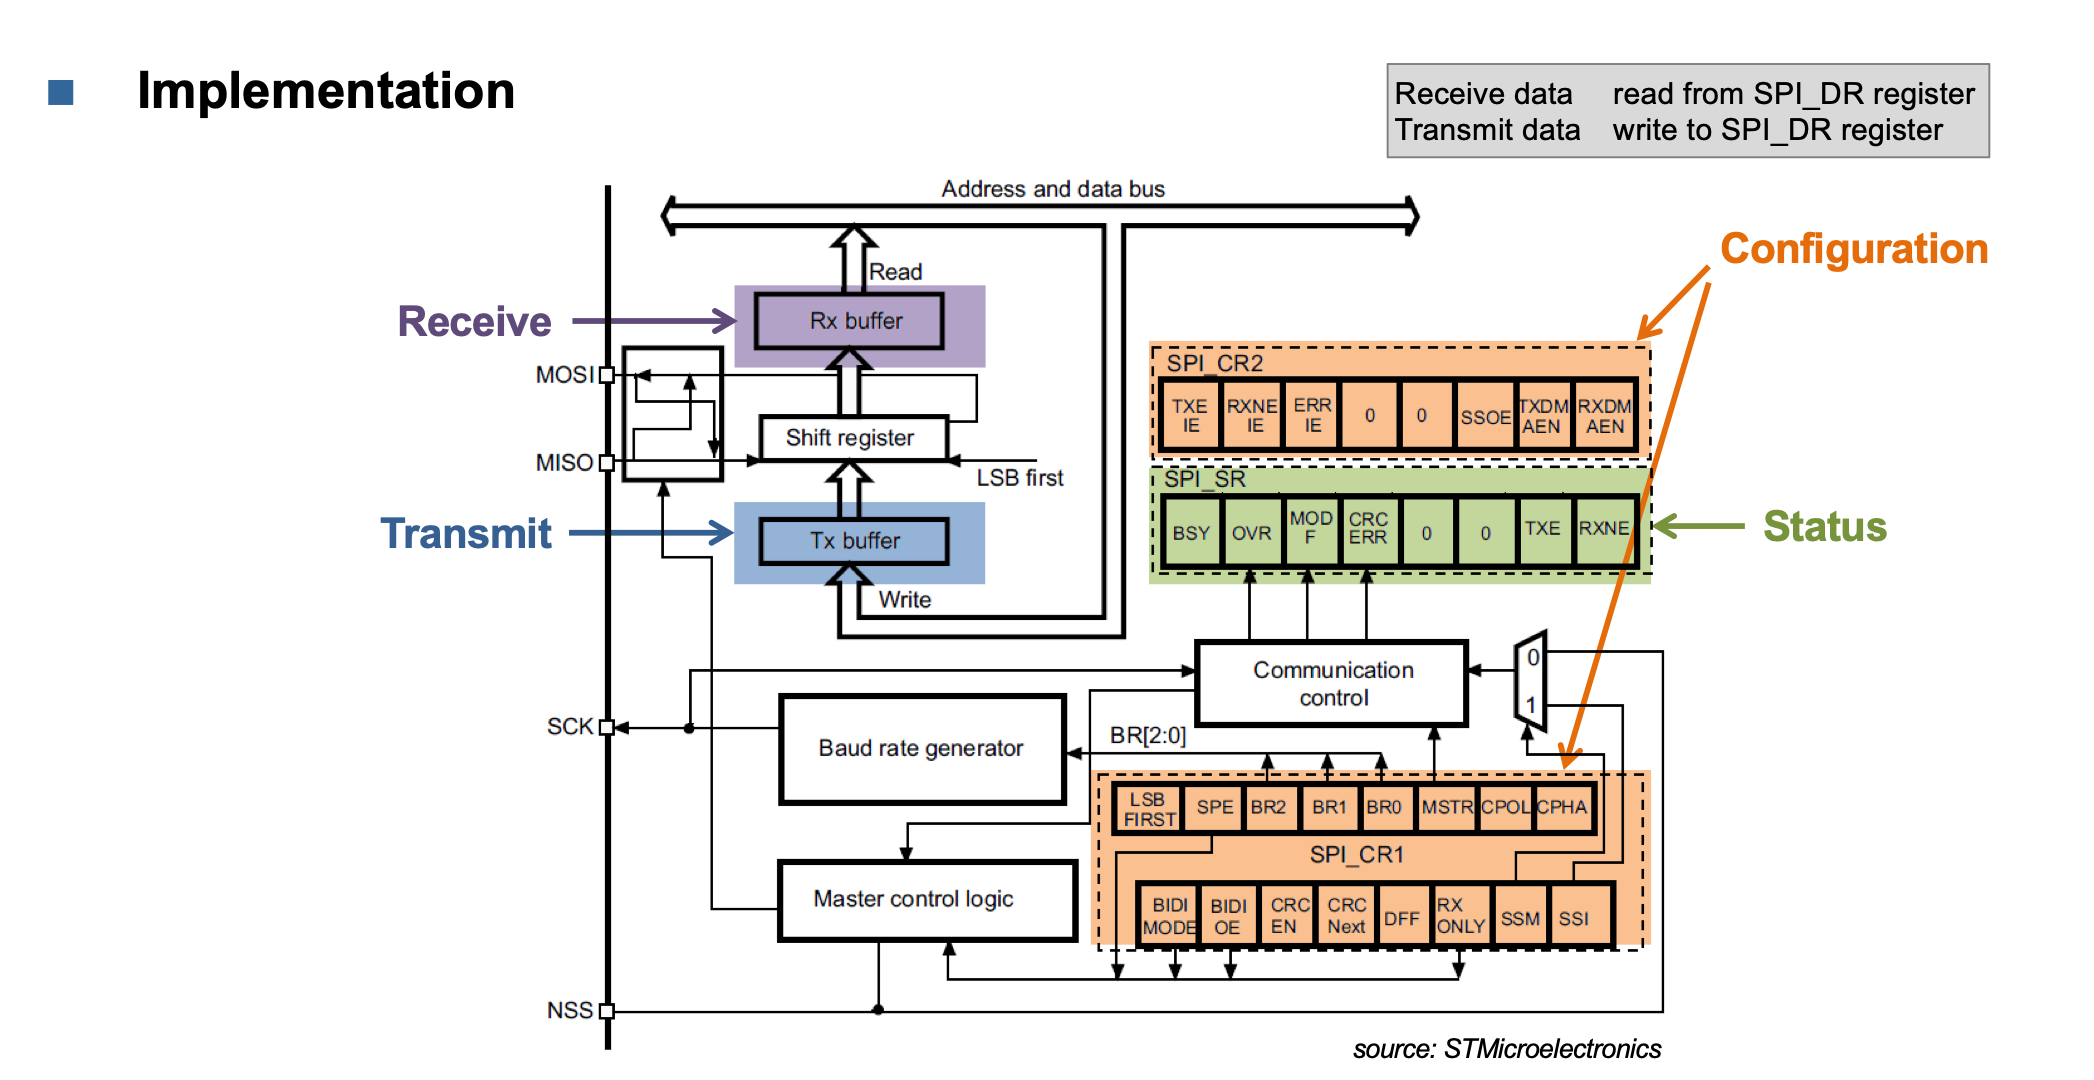
\includegraphics[width=0.3\textwidth]{sections/images/spi_impl.png}
\subsubsection{Synchronisierung von Hardware und Software}

\begin{itemize}
    \item TXE: Transmit Buffer Empty, Software kann nächstes TX Byte in Register SPI\_DR schreiben
    \item RXNE: Receive Buffer Not Empty, Software kann nächstes RX Byte aus Register SPI\_DR lesen
\end{itemize}

\subsubsection{Beispiel: SPI-Übertragung}
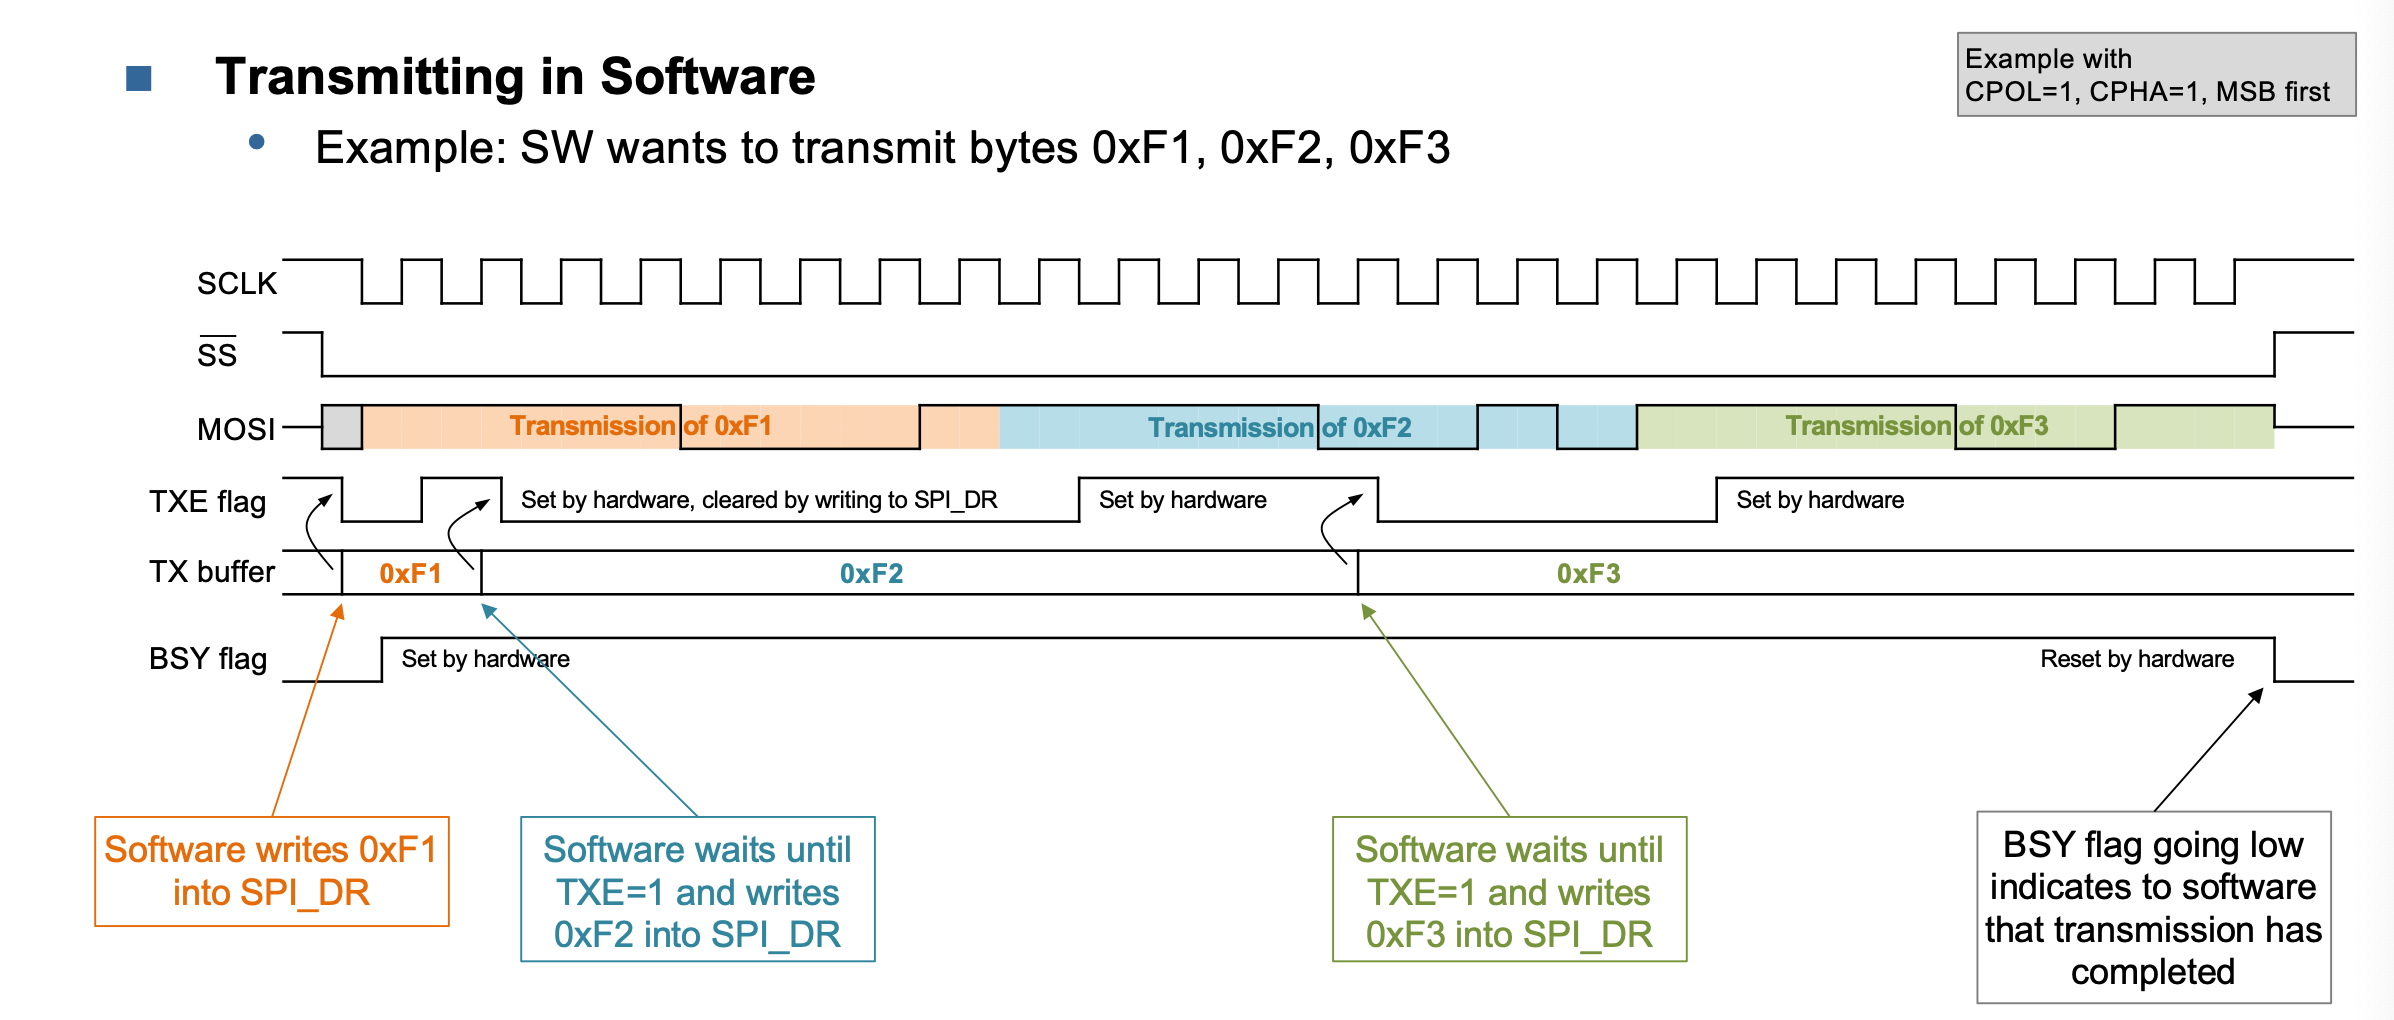
\includegraphics[width=0.3\textwidth]{sections/images/spi_example.png}
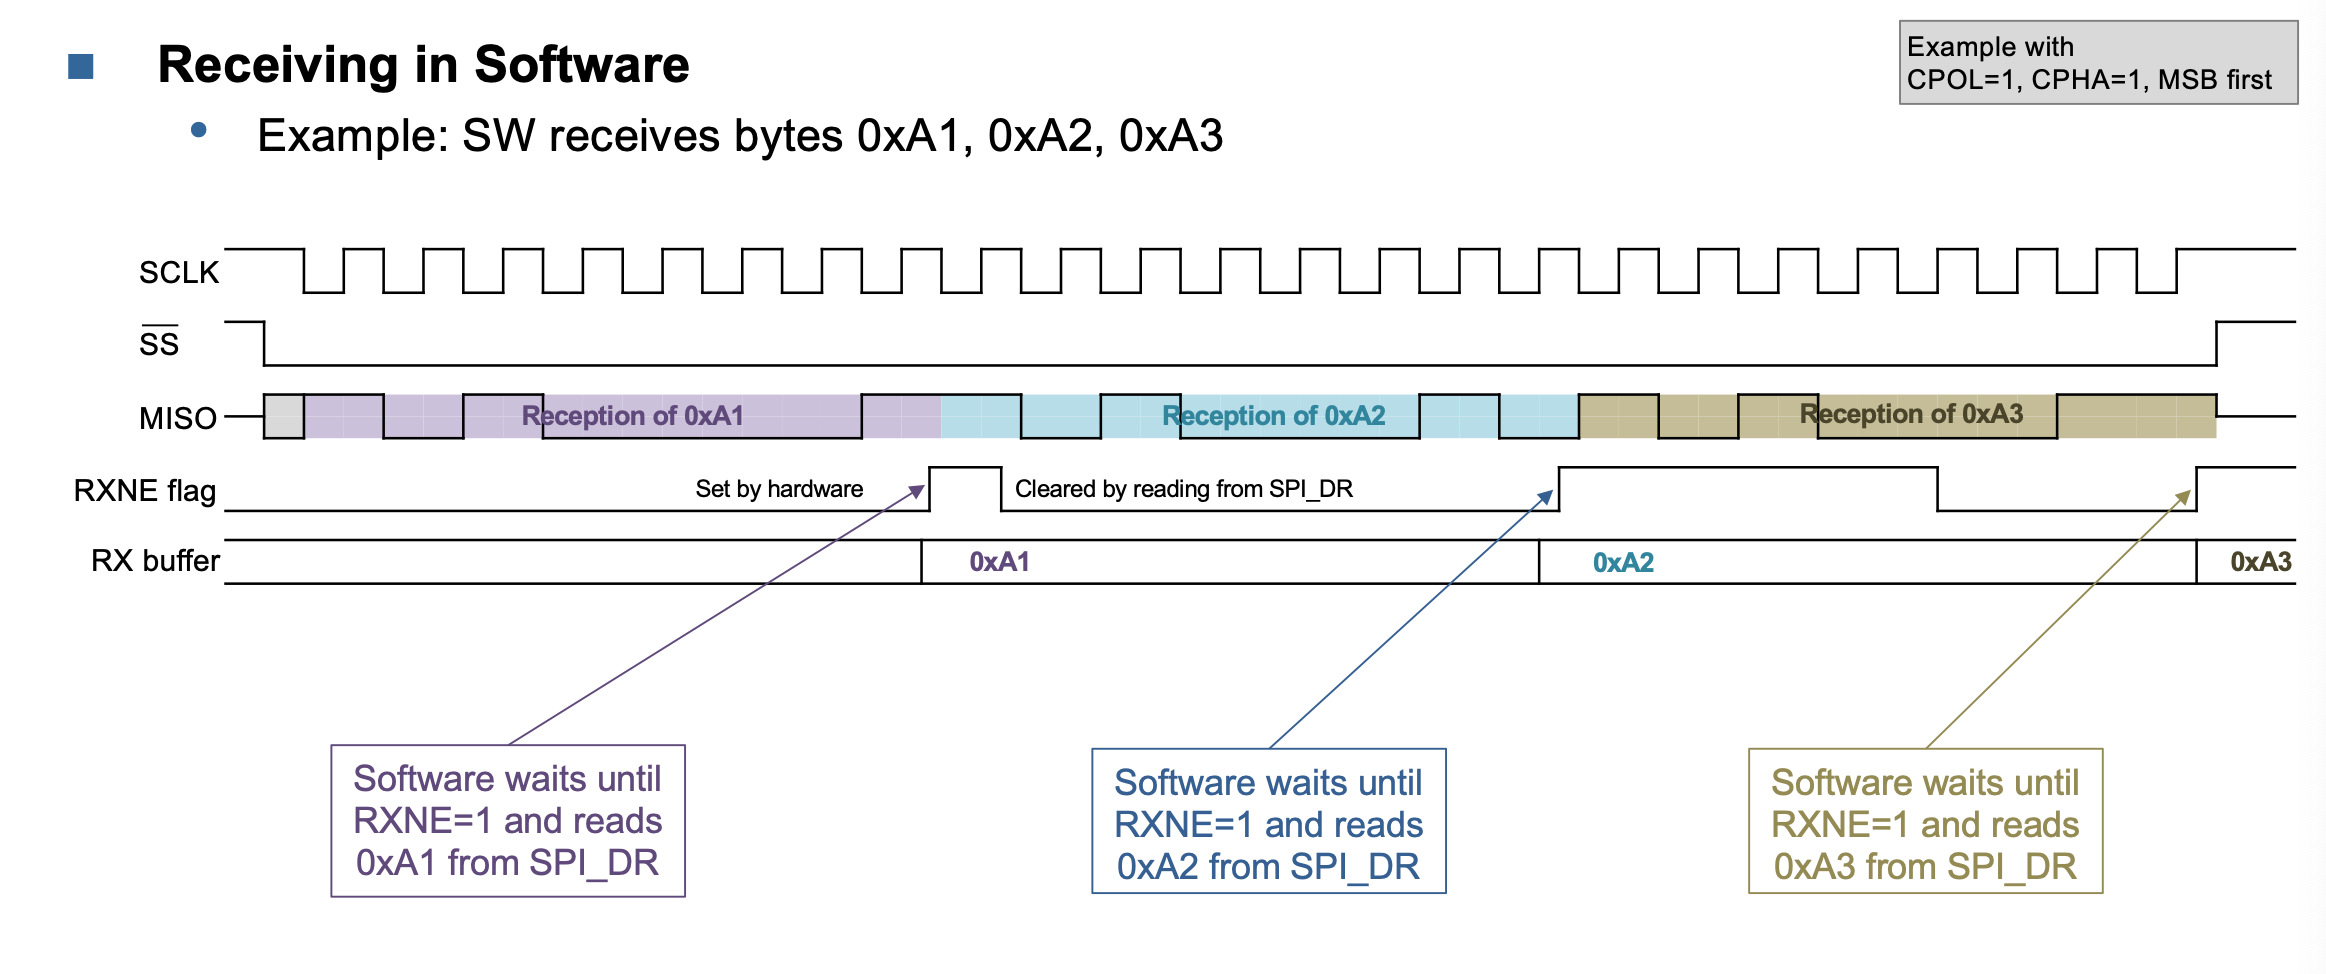
\includegraphics[width=0.3\textwidth]{sections/images/spi_example2.png}
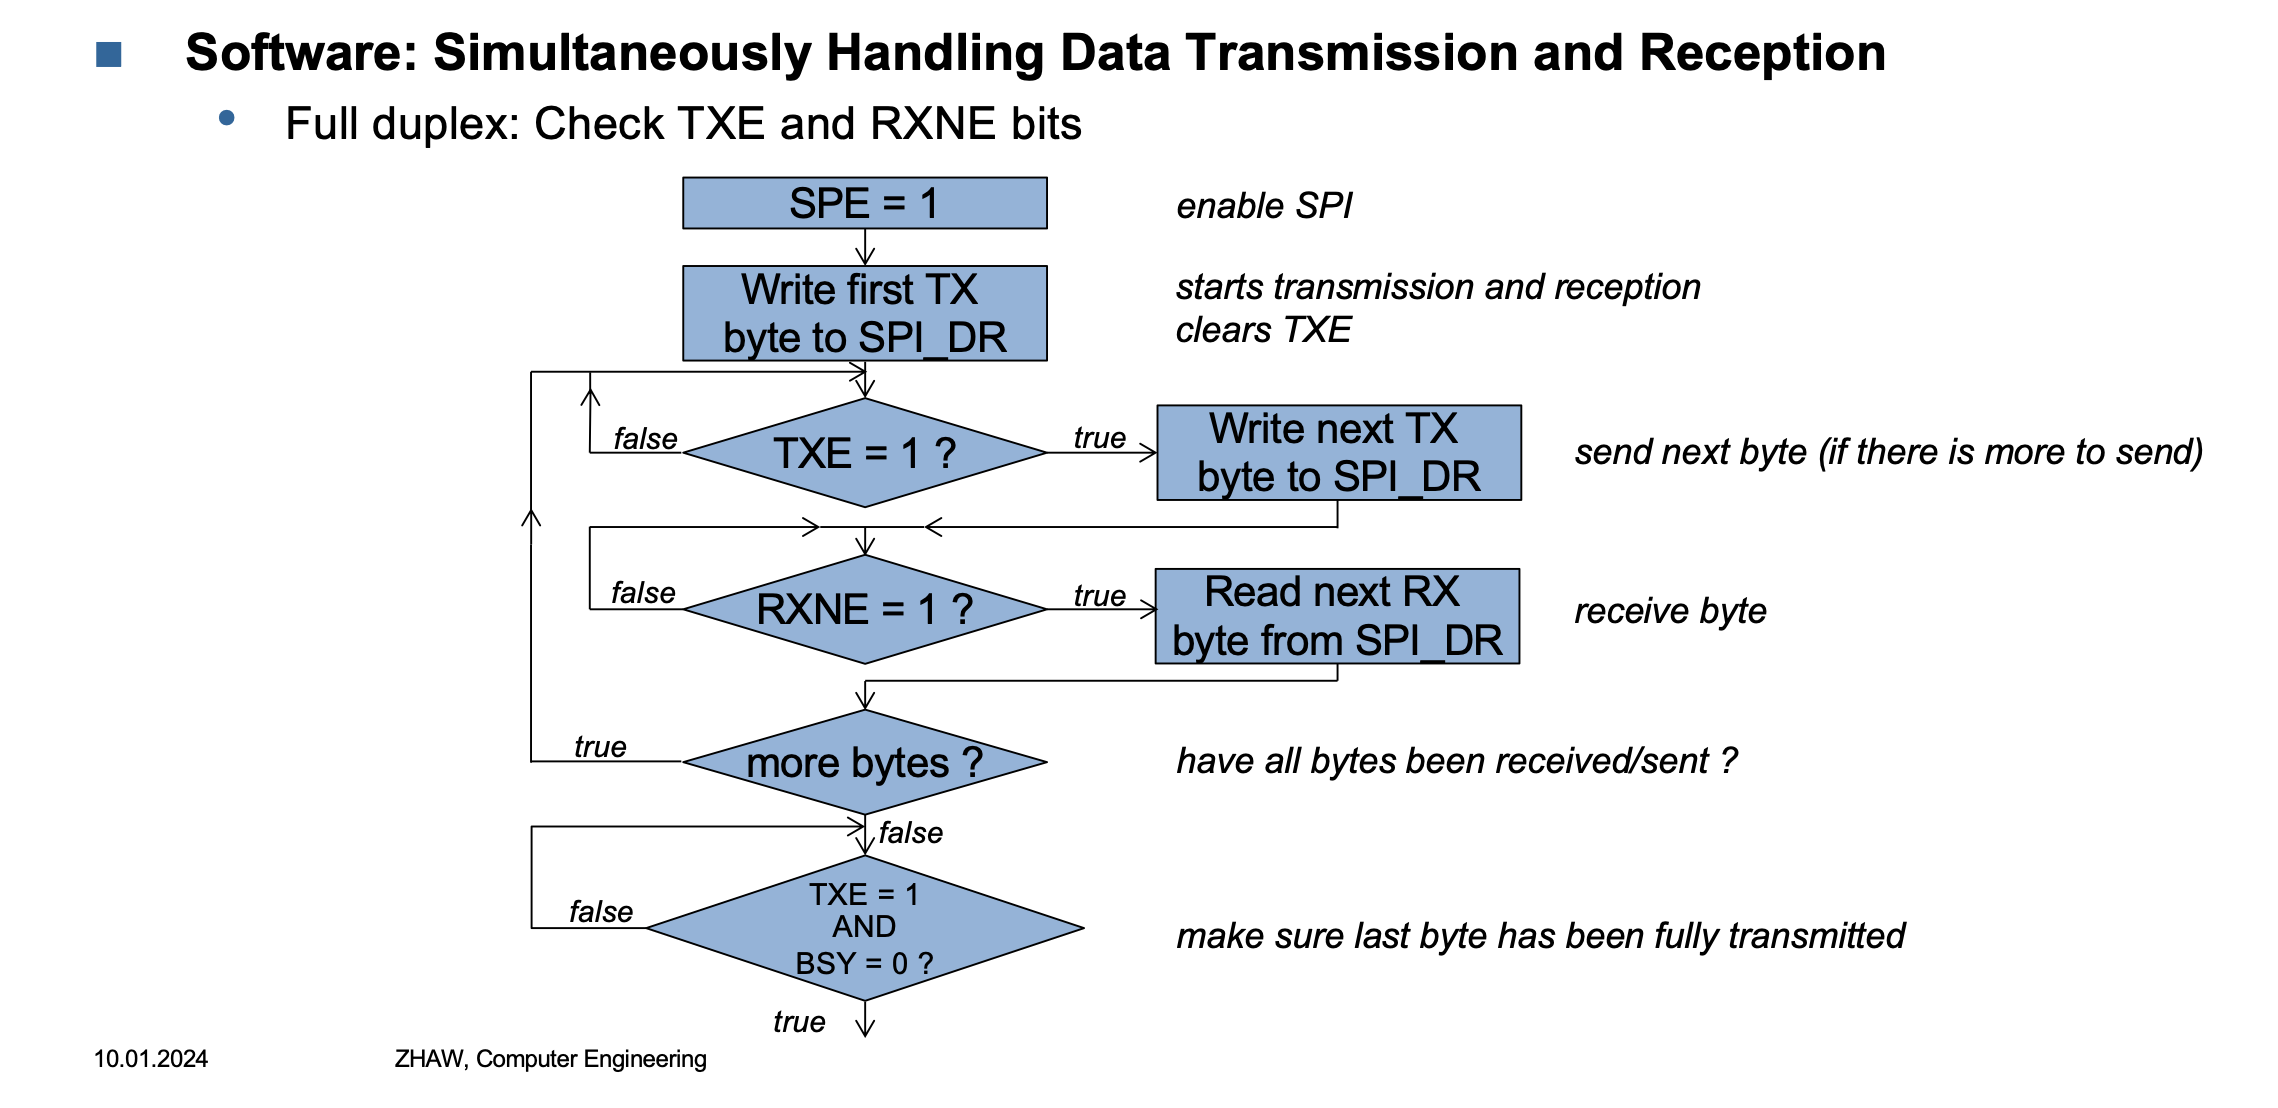
\includegraphics[width=0.3\textwidth]{sections/images/spi_sim.png}

\subsection{SPI Register}
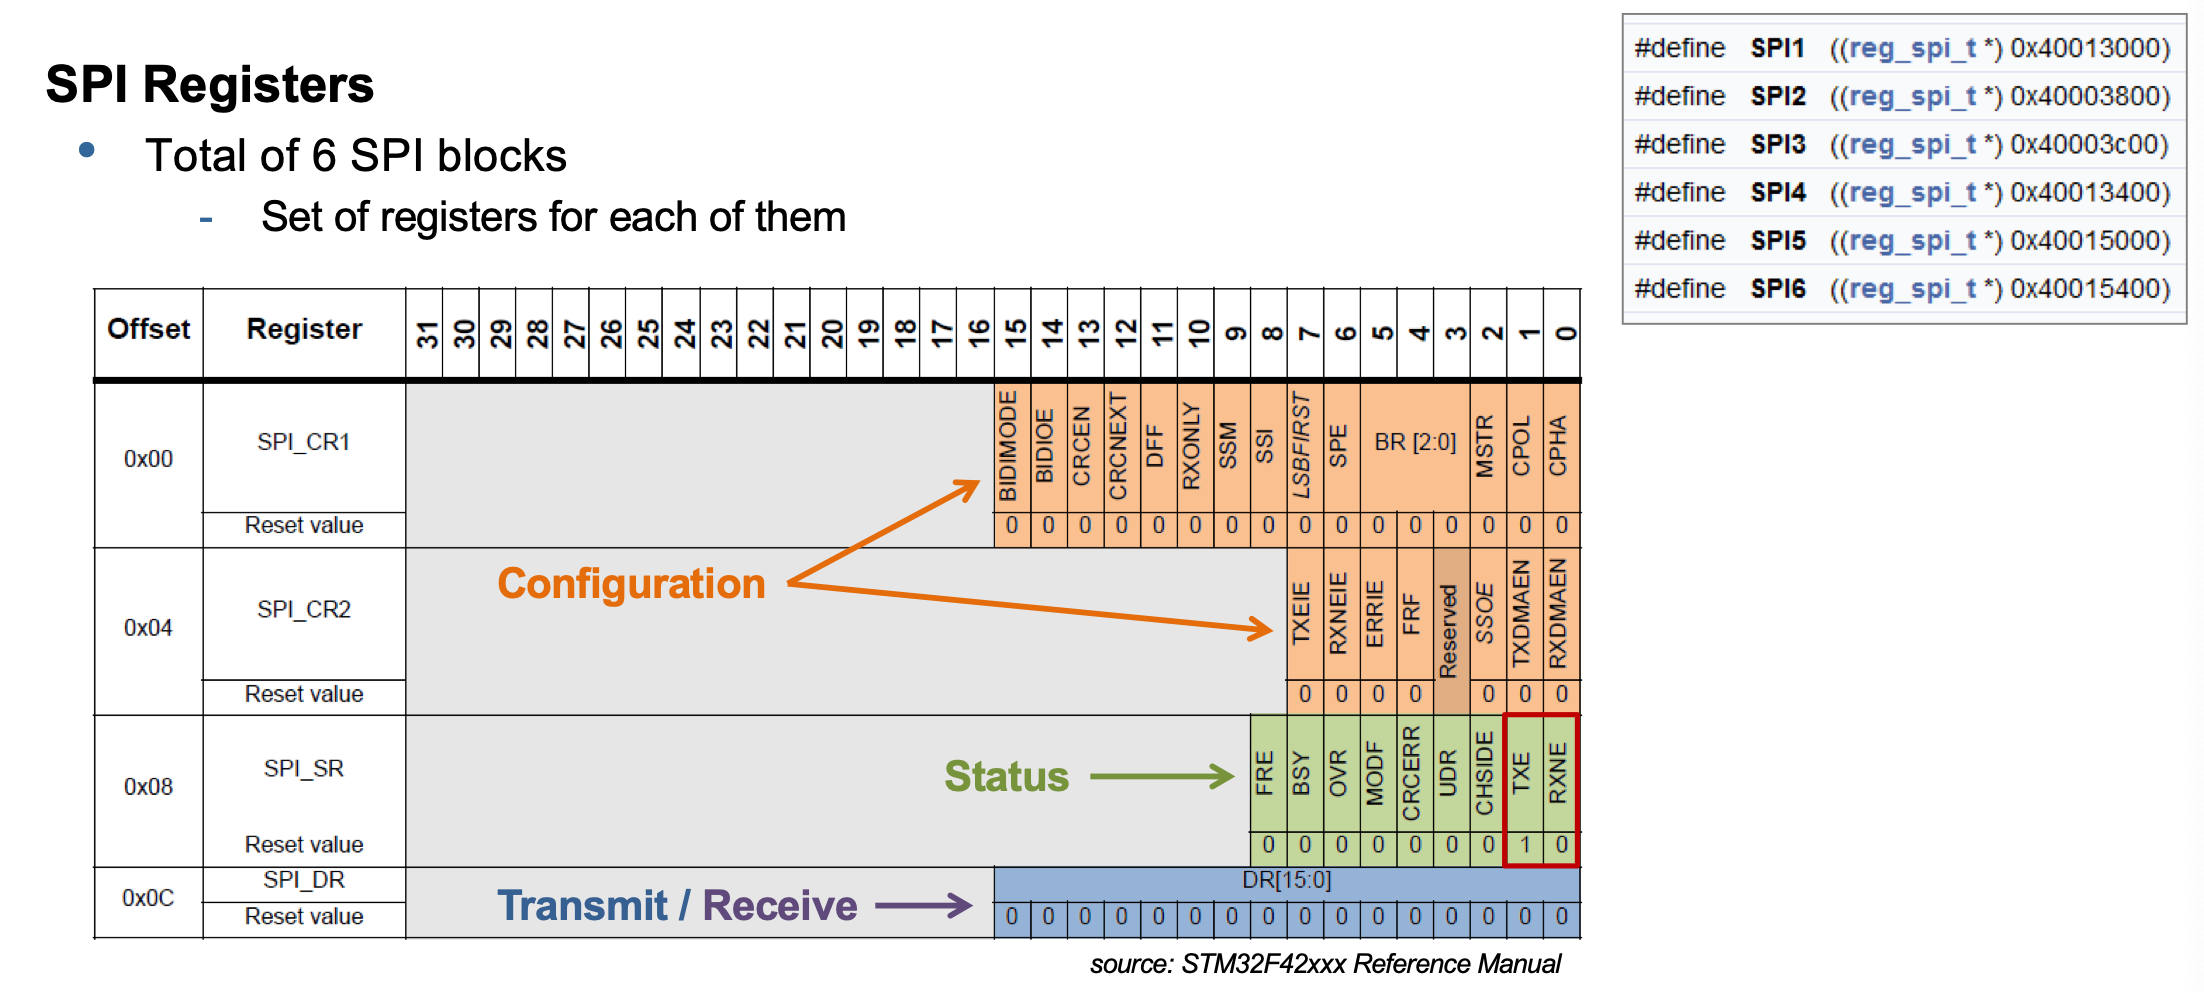
\includegraphics[width=0.3\textwidth]{sections/images/spi_register.png}
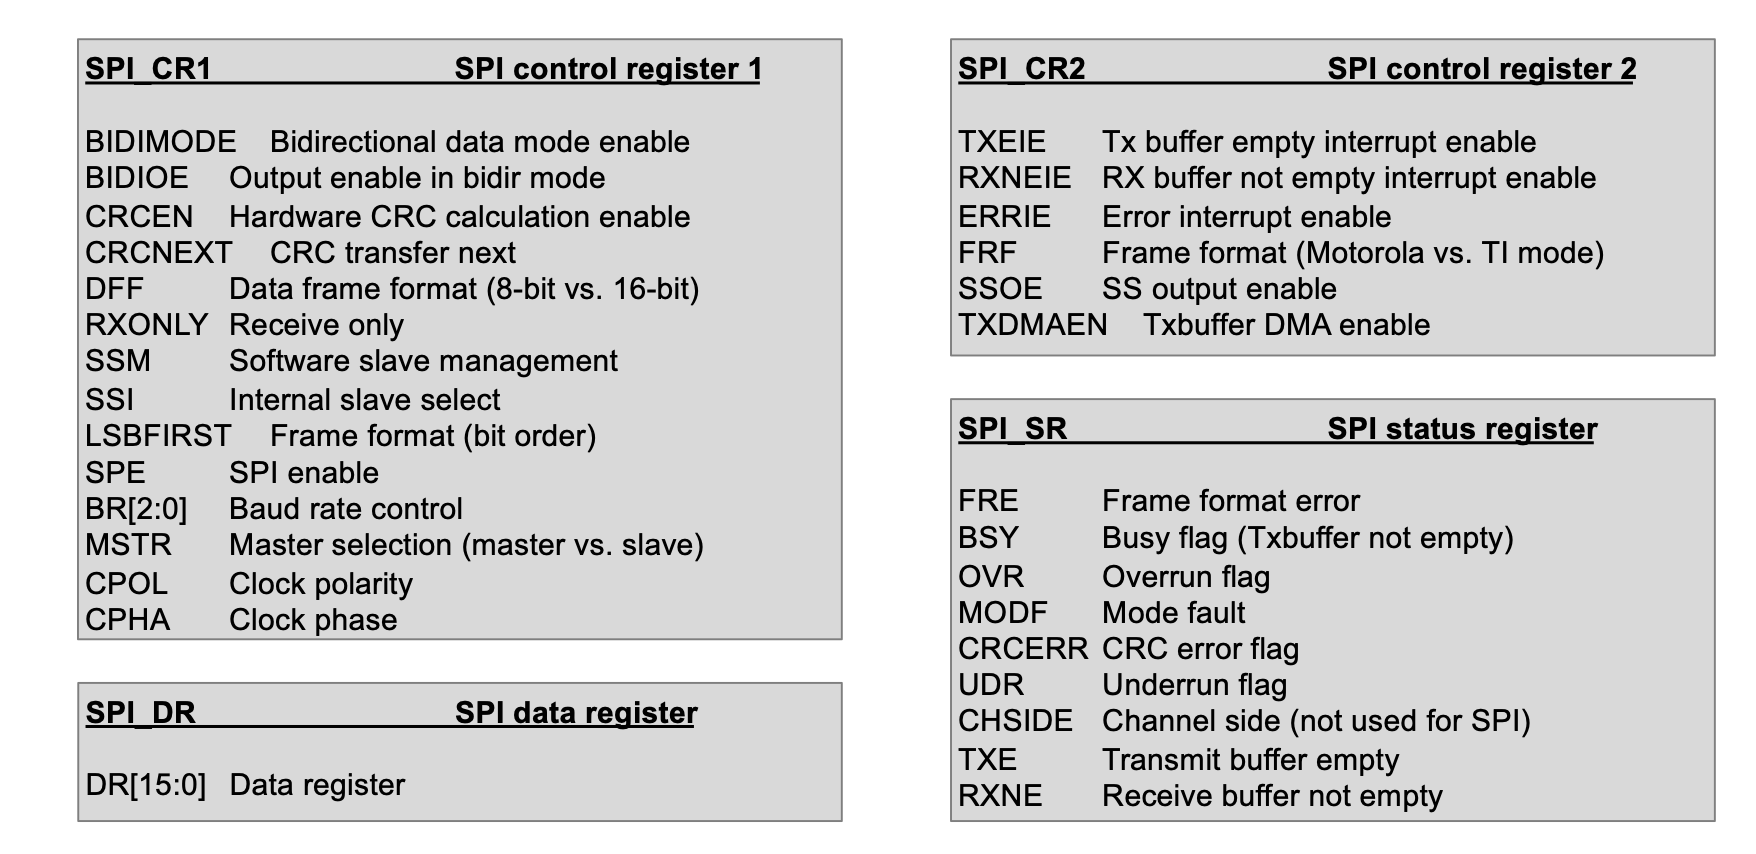
\includegraphics[width=0.3\textwidth]{sections/images/spi_register_bits.png}